% Main-paper qualitative figure: \input after macros.tex. Rendered by paper/figures/make_showcase.py from the test-split
% showcase assets (scripts/qual_assets.py --showcase); random draws are in appendix_qualitative.tex.
\begin{figure*}[t]
  \centering
  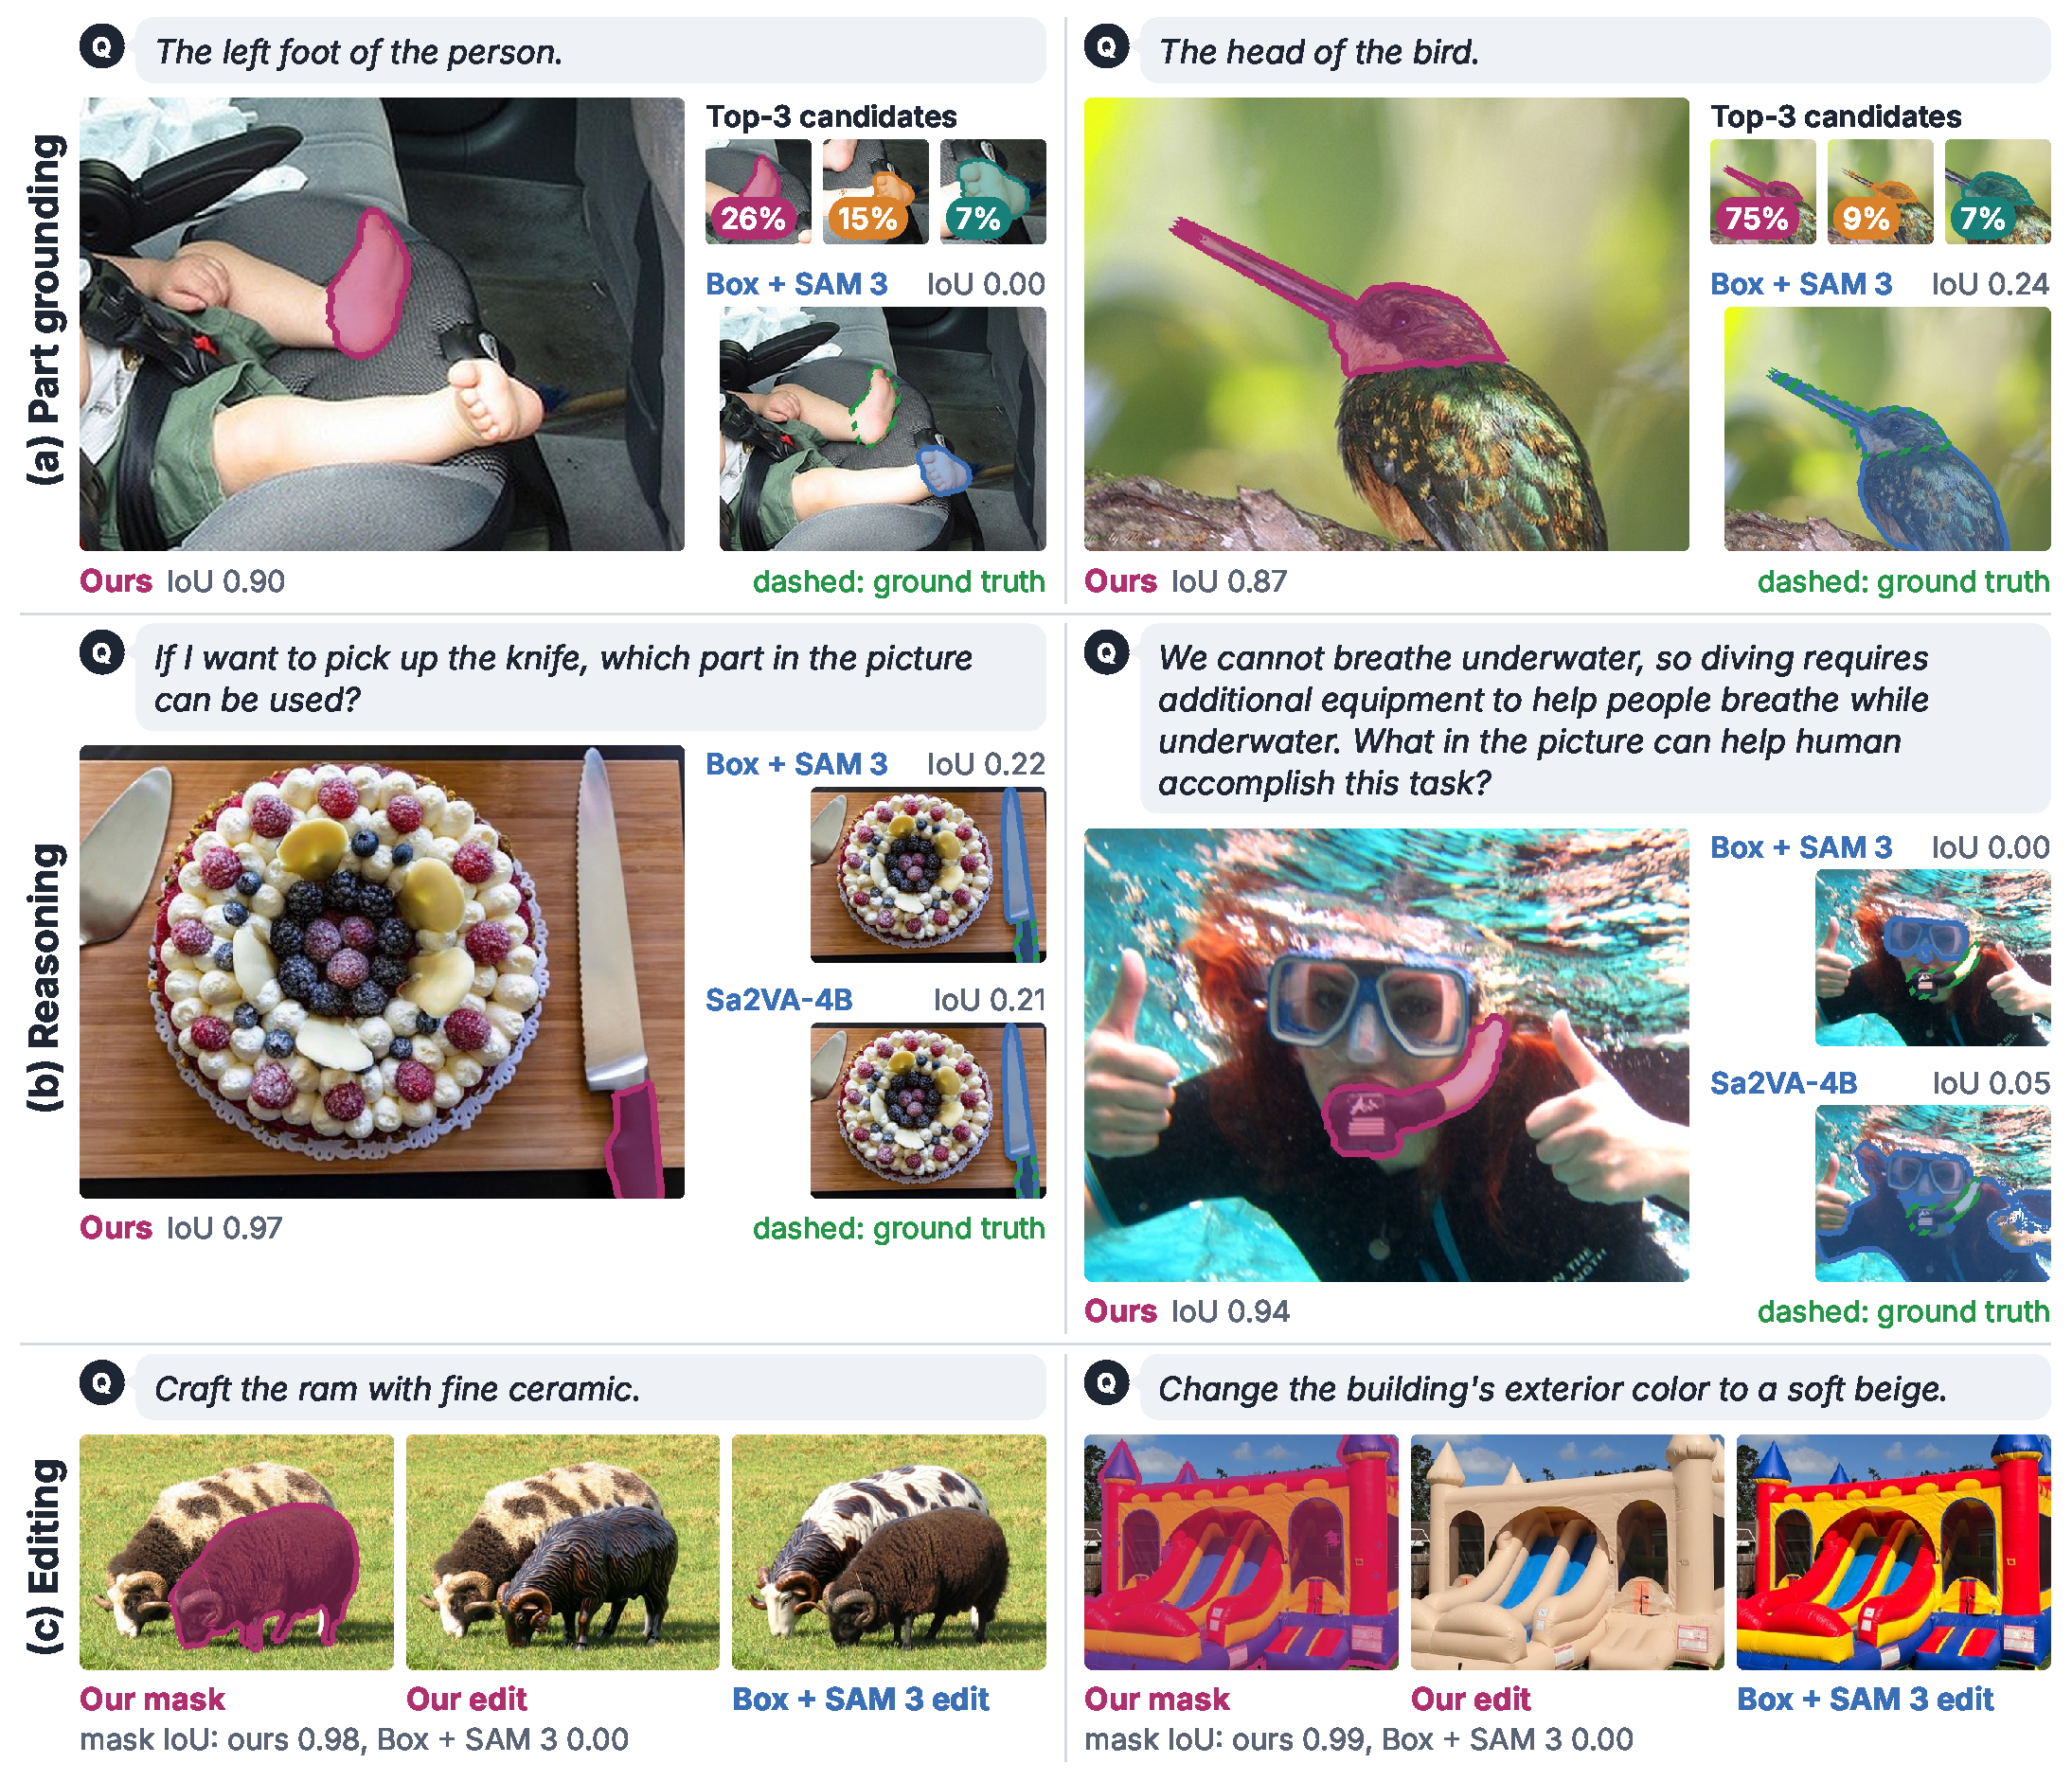
\includegraphics[width=\linewidth]{figures/qualitative/showcase.pdf}
  \caption{\textbf{Selected test examples.} Every method uses Qwen3-VL-4B. Filled magenta: the mask \ours{} selects; blue:
  Box + SAM\,3 (and Sa2VA-4B in~(b)); dashed green: ground truth. IoU is per query.
  (a)~Part grounding (Pascal-Part, PartImageNet); thumbnails show the three candidates \ours{} ranks highest, with
  their share of the selection softmax over the pool. Box + SAM\,3 returns the other foot or the whole bird.
  (b)~Reasoning (InstructPart, ReasonSeg), with query rewriting (\cref{sec:experiments}).
  (c)~Editing with Qwen-Image-Edit: the same instruction and editor, given our mask or the Box + SAM\,3 mask.
  The examples were chosen as clear wins; random examples, including failures, are in the supplementary material.}
  \label{fig:showcase}
\end{figure*}
